\Chapter{Resultaten\label{hfdst-resultaten}}

In dit hoofdstuk zal het ASIC ontwerp van de schakeling die in \refhfdst{hfdst-implementatie} beschreven werd van naderbij bestudeerd worden. Daarbij zal gekeken worden naar de oppervlakte van de schakeling, het verbruik en de maximum bereikbare kloksnelheid $f_{\text{max}}$. Er zal onderzocht worden wat het effect van de verschillende voorgestelde optimalisaties is op al deze parameters. Ten slotte zal het ontwerp vergeleken worden met reeds bestaande implementaties.

Het ontwerp werd geprogrammeerd in GEZEL \cite{gezel}. Simulaties en compilatie naar VHDL werden uitgevoerd met GEZEL 2.0. De optimalisaties werden doorgevoerd in de VHDL code, aangezien GEZEL dit niet toelaat. Alle ontwerpen werden gesynthetiseerd met behulp van Synopsys Design Vision. De gebruikte bibliotheek was de \emph{$0.13 \mu m$ low leakage} bibliotheek van Faraday Technology \cite{cell-databook}. De maximale oppervlakte werd ingesteld op nul, wat als netto effect een resultaat met minimum oppervlakte gaf. Verder werd voor het kloksignaal, zolang niet anders vermeld, een frequentie van 10kHz gedefini\"eerd.

De grootte van alle resultaten wordt uitgedrukt in gates. Dit laat toe te vergelijken met andere resultaten die in de literatuur terug te vinden zijn.

Voor de resultaten in verband met energieverbruik worden steeds twee waarden gegeven. De eerste waarde, dynamisch verbruik, geeft weer hoeveel vermogen verbruikt wordt door veranderende CMOS in- en uitgangen. De tweede waarde, leakage verbruik, is verbruik dat voorkomt zelfs indien een transistor niet geleidt. De impact hiervan hangt onder meer af van de gebruikte bibliotheek. Het is voor het synthese programma zeer moeilijk een nauwkeurige schatting voor het verbruik te geven, dus de gegeven waarden moeten niet als exact worden beschouwd.

% TODO: Blijft leakage constant bij hogere kloksnelheid?

Indien gewenst kan het verbruik voor hogere kloksnelheiden geschat worden. Gegeven de standaard frequentie $f = 10$kHz, de formule voor het dynamisch verbruik van een CMOS schakeling:
\[P_d = V^2 \cdot C \cdot f\]
en het leakage verbruik $P_l$, kan men dus het totale verbruik omrekenen naar dat van een willekeurige kloksnelheid via
\[P' = \frac{P_d \cdot f'}{10 \cdot 10^3} + P_l.\]
Het verkregen resultaat zal niet volledig zal kloppen, maar is meer dan goed genoeg om een schatting te kunnen maken van het totale verbruik.

\section{Benodigde rekentijd}

Alvorens de syntheseresultaten te presenteren, wordt even uitgewijd over het noodzakelijk aantal klokcycli $c$ om \'e\'en pairing te berekenen. Merk op dat de formules die volgen enkel kloppen voor willekeurige $m$ indien $\textsf{Hamm}(l) = 3$, wat het geval is voor de gekozen parameters (zie \refsect{sectie-implementatie-parameters}).

Het totaal aantal cycli wordt gegeven door:
\[c = 21681 + 4322 + 2998 \cdot \left\lceil \frac{m}{d} \right\rceil.\]
Daarbij staat het eerste getal voor het aantal klokcycli waarin geheugen van plaats verschoven wordt. Het tweede getal is het aantal optellingen dat uitgevoerd dient te worden en de co\"efficient voor de vermenigvuldiging is het aantal vermenigvuldigingen. Het aantal klokcycli $c$ kan verder opgesplitst worden in het aantal cycli $c_f$ voor de for-lus en $c_m$ voor de finale machtsverheffing. In dat geval zijn de formules:
\[\begin{gathered}
c_f = 18731 + 3937 + 2463 \cdot \left\lceil \frac{m}{d} \right\rceil\\
c_m = 2950 + 385 + 535 \cdot \left\lceil \frac{m}{d} \right\rceil,
\end{gathered}\]
waarbij de co\"efficienten opnieuw voor respectievelijk geheugenverschuivingen, optellingen en vermenigvuldigingen staan.

In \reftbl{tabel-resultaten-multi-cycles} wordt voor enkele waarden getoond hoeveel klokcycli nodig zijn om een berekening te voltooien in het geval $m = 163$. In \reffig{figuur-resultaten-multi-cycles} wordt hetzelfde weergegeven, maar dan voor elke $d$ van 1 t.e.m.\ 163. Het is duidelijk dat de tijdsbesparing waar extra MALUs voor zorgen vrij snel teniet wordt gedaan door het aantal cycli dat niet door $d$ be\"invloed wordt.

\begin{table}[h]
	\caption{Aantal klokcycli $c$ nodig voor \'e\'en pairing i.f.v.\ het aantal MALUs $d$ voor $m = 163$}
	\label{tabel-resultaten-multi-cycles}

	\begin{narrow}{-1cm}{-1cm}
		\centering
		\begin{tabular}{lllllllll}
			\toprule
			$d$	& 1	& 2	& 3	& 4	& 6	& 8	& 16	& 32\\
			$c$	& $514\,677$	& $271\,839$	& $190\,893$	& $148\,921$	& $109\,947$	& $88\,961$	& $58\,981$	& $43\,991$\\
			\bottomrule	
		\end{tabular}
	\end{narrow}
\end{table}

\begin{figure}[h]
	\centering
		\fbox{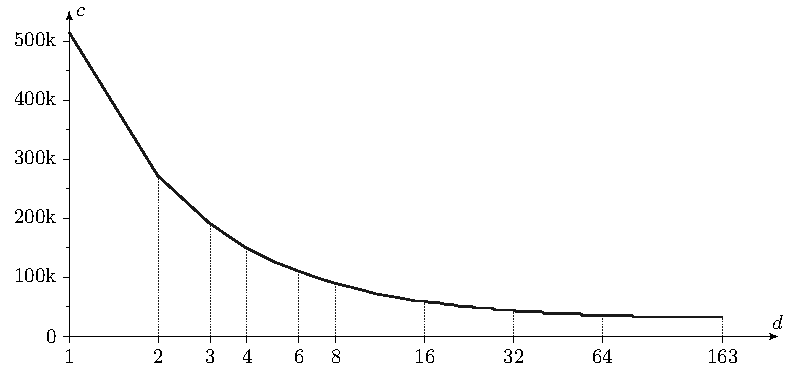
\includegraphics[width=11.9cm]{results-multi-cycles}}
		\caption{Aantal klokcycli $c$ nodig voor \'e\'en pairing i.f.v.\ het aantal MALUs $d$ voor $m = 163$\label{figuur-resultaten-multi-cycles}}
\end{figure}

\section{Basisimplementatie \& register optimalisaties\label{section-resultaten-basisimplementatie}}

Logischerwijs wordt eerst gekeken naar de syntheseresultaten voor een implementatie met \'e\'en MALU. Verder zal in deze paragraaf ook onderzocht worden wat de effecten zijn van de optimalisaties voorgesteld in \refsect{sectie-implementatie-optimalisaties}. Bij de implementaties met clock gating werden steeds ook de reset ingangen van zoveel mogelijk registers verwijderd. De synthese resultaten voor de vijf verschillende implementaties worden gegeven in \reftbl{tabel-resultaten-optimalisaties}. De versies met clock gating (CG~$n$) implementeren de schakelingen in de volgorde waarin ze voorkomen in \refsect{subsectie-implementatie-optimalisatie-clock-gating}. Ter verduidelijking zijn deze resultaten ook nog eens uitgezet in \reffig{figuur-resultaten-m1}.

%De synthese software gebruikt in de basis implementatie en die zonder reset ingangen flip flops met een enable ingang. Zo'n flip flops kosten achtentwintig gates, waarbij de reset ingang door twee van die gates gevormd wordt. Intern zijn deze flip flops equivalent aan een flip flop zonder enable ingang die naar zichzelf is terug gekoppeld via een multiplexer. Het enable signaal vervult in dit geval de functie van selectie signaal die anders voor de multiplexer nodig zou zijn. De synthese software zal zelf de sturing van de enable signalen bepalen in dit gevallen. Het is om deze reden dat het toepassen van clock gating in dit geval geen oppervlakte winst oplevert tegenover.

\begin{table}[h]
	\caption{Syntheseresultaten voor implementaties met \'e\'en MALU}
	\label{tabel-resultaten-optimalisaties}

	\centering
	\begin{tabular}{llrlrlr}
		\toprule
		\multirow{2}{*}{Ontwerp}	& \multicolumn{2}{l}{\multirow{2}{*}{Opp. [gates]}}	& \multicolumn{4}{c}{Verbruik @ 10kHz [$nW$]}\\
		\cmidrule{4-7}
		&	& & \multicolumn{2}{c}{Dynamisch}	& \multicolumn{2}{c}{Leakage}\\
		\midrule
		Basis			& $28\,876$	& 			& 512	&	 		& 117 & \\
		Geen Reset	& $27\,596$	& 96\%	& 395	& 77\%	& 107 & 92\%\\
		CG 1			& $27\,751$	& 96\%	& 94	& 18\%	& 109	& 94\%\\
		CG 2			& $27\,713$	& 96\%	& 59	& 12\%	& 102	& 88\%\\
		CG 3			& $27\,734$	& 96\%	& 96	& 19\%	& 110	& 94\%\\
		\bottomrule		
	\end{tabular}
\end{table}

\begin{figure}[h]
	\centering
		\fbox{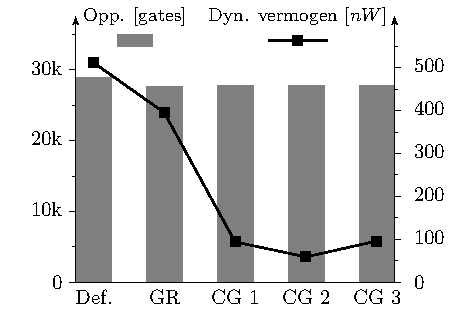
\includegraphics[scale=1]{results-m1}}
		\caption{Syntheseresultaten voor implementaties met \'e\'en MALU en $f = 10$kHz\label{figuur-resultaten-m1}}
\end{figure}

Zoals verwacht resulteert het toepassen van clock gating in een zeer grote besparing op het verbruik. Het is zelfs zo dat na toepassing van clock gating het dynamisch verbruik lager is dan het leakage verbruik. Daarbij dient opgemerkt te worden dat het dynamisch verbruik zal stijgen bij een hogere kloksnelheid terwijl het leakage verbruik constant zal blijven.

Het is opmerkelijk dat het dynamisch verbruik van CG~3 niet lager is dan dat van de andere twee CG implementaties. Dit mogelijk als volgt te verklaren: clock gating methode drie bespaart enkel energie tegenover de andere methodes indien de ingang van een register wijzigt wanneer dat register geen nieuwe waarde moet opslaan. De enige ingang die echter vaak wijzigt is die van het register verbonden met de uitgang van de $\mathbb{F}_{2^m}$ kern tijdens een vermenigvuldiging. Zolang een vermenigvuldiging aan de gang is, moet ditzelfde register echter telkens zijn eigen waarde verschoven met \'e\'en positie naar links opslaan. Met andere woorden: op het moment dat de clock gating schakeling zijn besparende werk zou kunnen verrichten, wordt het register sowieso elke klokslag beschreven met een nieuwe waarde. Het effect is dus dat in dit geval de schakeling effectief geen of amper vermogensbesparing teweeg brengt tegenover de andere clock gating schakelingen. Verder is het ook goed mogelijk dat de synthese software bij het berekenen van het verbruik niet nauwkeurig genoeg tewerk gaat om het effect van de schakeling op de interne gates van de flip flop in rekening te kunnen brengen.

Ten slotte wordt nog ontleed hoeveel oppervlakte de individuele onderdelen van de schakeling innemen. \reftbl{tabel-resultaten-onderdelen} geeft een overzicht van de grootte van de verschillende delen van implementatie CG~3. Het valt op dat de zestien registers en de FSM (logica van de controller) samen goed zijn voor 95.5\% van de oppervlakte. Het effect daarvan zal duidelijk worden in de volgende paragraaf, wanneer meerdere MALUs ge\"implementeerd worden.

\begin{table}[h]
	\caption{Oppervlakte van de individuele onderdelen in de implementatie met \'e\'en MALU}
	\label{tabel-resultaten-onderdelen}

	\centering
	\begin{tabular}{llr}
		\toprule
		Onderdeel					& \multicolumn{2}{c}{Opp. [gates]}\\
		\midrule
		MALU				 			& 458			& 1.7\%\\
		$\mathbb{F}_{2^m}$ kern	&				& \\
		$\quad$ Logica				& 783			& 2.8\%\\
		$\quad$ Registers			& 962			& 3.5\%\\
		Controller					&				& \\
		$\quad$ Logica				& $13\,044$	& 47\%\\
		$\quad$ Registers			& $12\,487$	& 45\%\\
		\midrule
		Totaal						& $27\,734$	& 100\%\\
		\bottomrule		
	\end{tabular}
\end{table}


\section{Meerdere MALUs\label{sectie-resulaten-malus}}

Mits de toevoeging van extra MALUs is het, zoals aangetoond, mogelijk de totale rekeningtijd drastisch te verlagen. Hoewel het gebruik van meerdere MALUs de uiteindelijke schakeling vergroot en dat dus enigszins in gaat tegen de originele doelstelling, wordt hier toch onderzocht in welke mate de interessante parameters hierdoor juist worden be\"invloed.

Op de implementaties met meerdere MALUs werd steeds de derde clock gating techniek (en het verwijderen van reset ingangen) toegepast, aangezien dit in werkelijkheid de grootste energiebesparing teweeg zou moeten brengen. Implementaties met een aantal MALUs gaande van twee t.e.m.\ twee\"endertig werden gesynthetiseerd. Een nog hoger aantal MALUs zou immers compleet ingaan tegen de originele doelstelling. De resultaten van de synthese zijn te zien in \reftbl{tabel-resultaten-md} en \reffig{figuur-resultaten-md}. Het valt op dat, zoals verwacht, het toevoegen van een klein aantal extra MALUs weinig extra oppervlakte en verbruik met zich meebrengt en dus een aangeraden manier is om de snelheid van de schakeling op te drijven. Dit wordt verder onderzocht in de volgende paragraaf.

\begin{table}[h]
	\caption{Syntheseresultaten voor implementaties met $d$ MALUs}
	\label{tabel-resultaten-md}

	\centering
	\begin{tabular}{llrlrlrl}
		\toprule
		\multirow{2}{*}{$d$} & \multicolumn{2}{l}{\multirow{2}{*}{Opp. [gates]}}	& \multicolumn{4}{c}{Verbruik @ 10kHz [$nW$]}	& \multirow{2}{*}{$\begin{array}{@{}c@{}}\text{Tijds-}\\\text{winst}\end{array}$}\\
		\cmidrule{4-7}
		&	& & \multicolumn{2}{c}{Dynamisch}	& \multicolumn{2}{c}{Leakage}	&\\
		\midrule
		1			& $27\,734$	& 			& 96	& 			& 110	& 			& \\
		2			& $28\,423$	& 102\%	& 90	& 94\%	& 113	& 103\%	& 47.2\%\\
		3			& $29\,071$	& 105\%	& 103	& 107\%	& 118	& 107\%	& 62.9\%\\
		4			& $30\,278$	& 109\%	& 108	& 113\%	& 122	& 111\%	& 71.1\%\\
		6			& $30\,956$	& 112\%	& 112	& 117\%	& 127	& 115\%	& 78.6\%\\
		8			& $32\,782$	& 118\%	& 122	& 127\%	& 136	& 124\%	& 82.7\%\\
		16			& $37\,798$	& 136\%	& 162	& 169\%	& 163	& 148\%	& 88.5\%\\
		32			& $47\,833$	& 172\%	& 212	& 221\%	& 213	& 194\%	& 91.5\%\\
		\hline		
	\end{tabular}
\end{table}

\begin{figure}[h]
	\centering
		\fbox{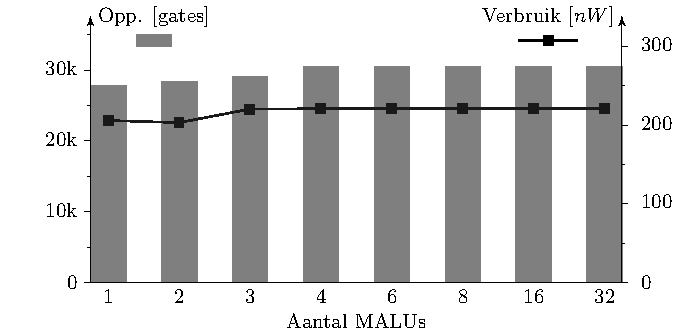
\includegraphics[scale=1]{results-md}}
		\caption{Syntheseresultaten voor implementaties met meerdere MALUs en $f = 10$kHz\label{figuur-resultaten-md}}
\end{figure}

\section{Hogere kloksnelheid vs.\ meerdere MALUs}

Aan de gegeven kloksnelheid $f = 10$kHz doet een schakeling met \'e\'en MALU er 51.5 seconden over om \'e\'en pairing te berekenen. Dit zal  in de meeste gevallen onaanvaardbaar zijn. Daarom wordt hier onderzocht wat de effecten op de schakeling zijn indien de kloksnelheid wordt opgedreven en er eventueel meerdere MALUs gebruikt worden. Ter illustratie zal voor een implementatie met meerdere MALUs die met twee nader onderzocht worden. Opnieuw wordt in beide gevallen clock gating schakeling drie gebruikt en worden zoveel mogelijk reset ingangen verwijderd.

Stel een maximale rekentijd $t_{\text{max}} \approx 50ms$. Voor een implementatie met \'e\'en MALU moet de klokfrequentie $f_1$ dan 1030 maal verhoogd worden. Wanneer men de schakeling met twee MALUs even snel wenst te maken als die met \'e\'en dan dient de kloksnelheid $f_2$ van die eerste vermenigvuldigd te worden met $\Delta f = 1 - 0.472$.
%\[\begin{aligned}
%\Delta f &=  1 - 0.472\\
%	&= 0.528.
%\end{aligned}\]
De kloksnelheden van de respectievelijke schakelingen zijn dan:
\[\begin{aligned}
f_1	&\approx 10.3\text{MHz}\\
f_2	&\approx 5.44\text{MHz}.
\end{aligned}\]

Ter vergelijking worden de resulterende parameters van beide implementaties gegeven in \reftbl{tabel-resultaten-m1-vs-m2}. Beiden werden gehersynthetiseerd met aangepaste parameters voor de klok. Dat de schakeling met \'e\'en MALU in dit geval kleiner is dan in het geval $f = 10$kHz, is te wijten aan enige willekeurigheid in de algoritmes van de synthesesoftware. Hoewel de implementatie met twee MALUs 3\% groter is dan die met \'e\'en, verbruikt ze slechts de helft zoveel vermogen. Het lijkt dus vanzelfsprekend om steeds voor een implementatie met meerdere MALUs te kiezen indien de snelheid moet opgedreven worden. Hoeveel MALUs ideaal zijn, zal afhankelijk zijn van toepassing tot toepassing.

\begin{table}[h]
	\caption{Vergelijking van syntheseresultaten voor twee verschillende implementaties die er even lang over doen \'e\'en pairing te berekenen}
	\label{tabel-resultaten-m1-vs-m2}

	\centering
	\begin{tabular}{lll@{$\;\;$}l}
		\toprule
		& 1 MALU	& \multicolumn{2}{l}{2 MALUs}\\
		\midrule
		$f$ [MHz]					& 10.3						& 5.44						& 53\% \\ 
		Opp. [gates]				& $27\,430$					& $28\,155$					& 103\% \\
		Verbruik [$\mu W$]		& 								& 								& \\
		$\quad$ Dynamisch			& 98.2						& 48.5						& 49\% \\
		$\quad$ Leakage			& $107 \cdot 10^{-3}$	& $111 \cdot 10^{-3}$	& 104\% \\
		\bottomrule	
	\end{tabular}
\end{table}

\section{Vergelijking met bestaande implementaties}

Gezien de vrij recente ontdekking van pairings is het beschikbare aantal implementaties voor ASICs ook vrij beperkt. Er werden slechts drie papers in de literatuur gevonden waarin het voorgestelde ontwerp naar een ASIC gesynthetiseerd werd. Enkele papers beschrijven een ontwerp voor gebruik in sensor netwerken. Helaas hebben deze als doelplatform allemaal een microprocessor. Zowat alle andere gepubliceerde implementaties werden ontwikkeld in software of voor FPGAs. Verder wordt in het geval van de FPGA ontwerpen, waar een zekere controle over de uiteindelijke grootte mogelijk is, zowat steeds geoptimaliseerd naar een minimum oppervlakte rekentijd product. Voor laag vermogensschakeling is dit echter geen interessante waarde. Het is dus zowat onmogelijk een grondige vergelijking te maken tussen de verschillende bestaande implementaties. Toch zal zo goed als mogelijk getracht worden een overzicht te geven, zodat het in deze thesis voorgestelde ontwerp beter geplaatst kan worden.

\subsection{Microchip implementaties}

Implementaties van pairings voor gebruik op een MICA node, specifiek ontwikkeld voor gebruik in sensor netwerken, worden voorgesteld in \cite{tinytate}, \cite{tinypbc} en \cite{nanoecc}. De processor op deze nodes is een ATMega128L microchip. Een overzicht van de resultaten is gegeven in \reftbl{tabel-resultaten-sensor}. Rekening houdend met het stroomverbruik gegeven in \cite{nanoecc} wordt het verbruik geschat op ongeveer $23.60mW$. Uiteraard zijn de oppervlakte en het verbruik van een microchip implementatie niet te vergelijken met de in deze thesis voorgestelde ASIC implementatie, gezien de zeer verschillende architectuur van en filosofie achter de keuze voor beiden.

\begin{table}[h]
	\caption{Resultaten uit de literatuur voor implementaties met focus op sensor netwerken}
	\label{tabel-resultaten-sensor}

	\centering
	\begin{tabular}{lllll}
		\toprule
		& \multirow{2}{*}{TinyTate \cite{tinytate}}	& \multirow{2}{*}{TinyPBC \cite{tinypbc}} &	\multicolumn{2}{c}{NanoECC \cite{nanoecc}}\\
		\cmidrule{4-5}
		& & & \multicolumn{1}{c}{Binair} & \multicolumn{1}{c}{Priem}\\
			\midrule
		Veld					& $\mathbb{F}_{p}$ 256 bit	& $\mathbb{F}_{2^{271}}$	& $\mathbb{F}_{2^{163}}$	& $\mathbb{F}_{p}$ 160 bit\\
		Pairing				& Tate							& $\eta_T$ 						& Tate							& Tate\\
		Rekentijd ($s$)	& 30.21							& 5.45							& 10.96							& 17.93\\
		\bottomrule
	\end{tabular}
\end{table}

\subsection{FPGA implementaties}

In de literatuur zijn vrij veel ontwerpen voor FPGAs terug te vinden. Het probleem is echter dat men zich bij het ontwerp hiervan steeds toelegt op het behalen van een zo hoog mogelijke snelheid, wat resulteert in een grote oppervlakte. Ook wordt vaak gerekend over grotere velden dan hetgeen waarover gerekend wordt in deze thesis (bv. $\mathbb{F}_{2^{313}}$ of $\mathbb{F}_{3^{197}}$), wat meer veiligheid biedt, maar resulteert in nog grotere ontwerpen.

Grootte van een FPGA ontwerp wordt vermeld in \emph{slices} (Xilinx) of \emph{logic elements} (Altera). Deze eenheden zijn onmogelijk om te zetten naar een aantal gates. Zodoende is het dus niet mogelijk de grootte van deze ontwerpen te vergelijken met die van een ASIC schakeling.

Toch wordt in \reftbl{tabel-resultaten-fpga} een sumier overzicht gegeven van een zeer beperkt aantal ontwerpen. Bij de selectie hiervan werd vooral gekozen voor ontwerpen waarin in een vrij klein veld gerekend werd. Er dient in acht te worden genomen dat bij al deze implementaties snelheid, en niet oppervlakte, het voornaamste doel is. Het gebruik van een vermenigvuldigingsschakeling equivalent aan het gebruik van honderd of meer MALUs is in deze gevallen eerder regel dan uitzondering. Ook worden steeds meerdere berekeningen in parallel uitgevoerd.

\begin{table}[h]
	\caption{Resultaten uit de literatuur voor implementaties ontwikkeld voor FPGAs}
	\label{tabel-resultaten-fpga}

	\centering
	\begin{tabular}{llllll}
		\toprule
		&	\multicolumn{1}{c}{Veld}	& \multicolumn{1}{c}{Pairing}	& $\begin{array}{@{}c@{}}\text{Opp.}\\\text{[slices]}\end{array}$	& $\begin{array}{@{}c@{}}f\\\text{[MHz]}\end{array}$	& $\begin{array}{@{}c@{}}\text{Reken-}\\\text{tijd }[\mu s]\end{array}$\\
		\midrule
		Ronan \emph{et al.} \cite{ronan}				& $\mathbb{F}_{2^{103}}$	& Mod. Tate	& 21021	& 51	& 206\\
		Shu \emph{et al.} \cite{shu}					& $\mathbb{F}_{2^{239}}$	& Mod. Tate	& 25287	& 84	& 41\\
		Keller \emph{et al.} \cite{keller}			& $\mathbb{F}_{2^{251}}$	& Mod. Tate	& 27725	& 40	& 2370\\
		Grabher en Page \cite{grabher}				& $\mathbb{F}_{3^{97}}$		& Mod. Tate	& 4481	& 150	& 432\\
		Beuchat \emph{et al.} \cite{beuchat-eta}	& $\mathbb{F}_{3^{97}}$		& $\eta_T$	& 1833	& 145	& 192\\
		\bottomrule
	\end{tabular}
\end{table}

\subsection{ASIC implementaties}

Ten slotte rest dan nog de vergelijking met de tot nu toe gepubliceerde ASIC ontwerpen. De drie ontwerpen worden voorgesteld in respectievelijk \cite{beuchat-asic}, \cite{kammler} en \cite{savas}. Zowel in \cite{beuchat-asic} als \cite{savas} wordt met het oog op het behalen van zo hoog mogelijke snelheden ontworpen. De implementatie uit \cite{kammler} bevat naast de schakeling voor pairings tevens een RISC processor. In \cite{savas} wordt de finale machtsverheffing niet uitgevoerd. \reftbl{tabel-resultaten-asic} geeft een vergelijkend overzicht van het ontwerp voorgesteld in deze thesis en de vermelde ontwerpen. Aangezien het ontwerp uit \cite{beuchat-asic} het enige is waarvan alle gegevens bekend zijn, zal in de tekst die volgt enkel met dat ontwerp vergeleken worden. 

\begin{table}[h]
	\caption{Vergelijking van de implementatie voorgesteld in deze thesis met ASIC implementaties uit de literatuur}
	\label{tabel-resultaten-asic}

	\begin{narrow}{-2cm}{-2cm}
		\centering
		\begin{tabular}{llllll}
			\toprule
			&	\multicolumn{2}{c}{Thesis (1 MALU, CG 3)}	& \multirow{2}{*}{$\begin{array}{@{}c@{}}\text{Pairing-}\\\text{Lite \cite{beuchat-asic}}\end{array}$}	& \multicolumn{1}{c}{\multirow{2}{*}{$\begin{array}{@{}c@{}}\text{Kammler}\\\text{\emph{et al.} \cite{kammler}}\end{array}$}}	&  \multicolumn{1}{c}{\multirow{2}{*}{$\begin{array}{@{}c@{}}\text{K\"om\"urc\"u en}\\\text{Savas \cite{savas}}\end{array}$}}\\
			\cmidrule(r){2-3}
			& \multicolumn{1}{c}{$\begin{array}{@{}c@{}}d = 1,\\f = 10\text{kHz}\end{array}$} & \multicolumn{1}{c}{$\begin{array}{@{}c@{}}d = 2,\\f = 5.44\text{MHz}\end{array}$} & & &\\
	 		\midrule
			Veld																				& $\mathbb{F}_{2^{163}}$	& $\mathbb{F}_{2^{163}}$	& $\mathbb{F}_{3^{97}}$	& $\mathbb{F}_{p}$ 256 bit	& $\mathbb{F}_{3^{97}}$ \\
			Pairing																			& Tate							& Tate							& $\eta_T$					& Optimal Ate 					& Tate\\
			Technologie																		& $0.13 \mu m$					& $0.13 \mu m$					& $0.18 \mu m$				& $0.13 \mu m$					& $0.25 \mu m$\\
			Opp. [gates]																	& $27\,734$						& $28\,155$						& $193\,765$				& $97\,000$						& \emph{$10mm^2$}\footnotemark[2]\\
			$f$ [MHz]																		& 0.01							& 5.44							& 200							& 338								& 78\\
			Rekentijd [$\mu s$]															& $51.5 \cdot 10^6$			& $50 \cdot 10^3$				& 46.7						& $15.8 \cdot 10^3$			& 250\footnotemark[3]\\
			Verbruik [$mW$]																& $206 \cdot 10^{-6}$		& $48.6 \cdot 10^{-3}$		& 672							& ?								& ?\\
%			Score $\left[ mJ \cdot \text{gates} \right]$\footnotemark[4]	& 284								& 382								& 162							& ?								& ?\\
%			Score $\left[ \frac{nW}{\text{MHz} \cdot \text{gate}} \right]$\footnotemark[4]	& 0.74	& 0.32							& 17.34						& ?								& ?\\
			Score $\left[ \frac{\text{fJ}}{\text{gate}} \right]$\footnotemark[4]	& 0.74					& 0.32							& 17.34						& ?								& ?\\
			\bottomrule		
		\end{tabular}
	\end{narrow}
	
	\footnotesize \footnotemark[2] De gegeven oppervlakte is die van de complete schakeling inclusief routing.
	
	\footnotemark[3] Exclusief de finale machtsverheffing.
	
	\footnotemark[4] Des te lager de score, des te conservatiever springt de implementatie om met energie. De score wordt berekend als score $= \frac{\text{verbruik}}{\text{frequentie} \cdot \text{oppervlakte}}$. 
\end{table}

De hier voorgestelde implementaties zijn niet alleen ongeveer een factor zeven kleiner dan dat voorgesteld in \cite{beuchat-asic}, hun verbruik per gate (genormaliseerd voor frequentie) is ook beduidend lager. Uiteraard moet er wel op gewezen worden dat het ontwerp uit \cite{beuchat-asic} door het gebruik van een groter veld een grotere veiligheid biedt en, zoals reeds vermeld, niet ontworpen is met compactheid of laag verbruik in gedachten. Het is dus zeker niet de bedoeling het ontwerp af te breken. Het is echter wel duidelijk dat de ontwerpen voorgesteld in deze thesis met kop en schouders uitsteken boven dat van \cite{beuchat-asic} indien compactheid en laag vermogenverbruik prioriteit genieten.
